\chapter{Introduction}

\section{Background and Motivation}
{\color{red} 
	
	Below paragraph was taken from Advance Project-II and it will be used as a background information after summarizing.
	
	 \begin{figure}[!ht]
	\begin{center}
		\makebox[\textwidth]{
			\centering
			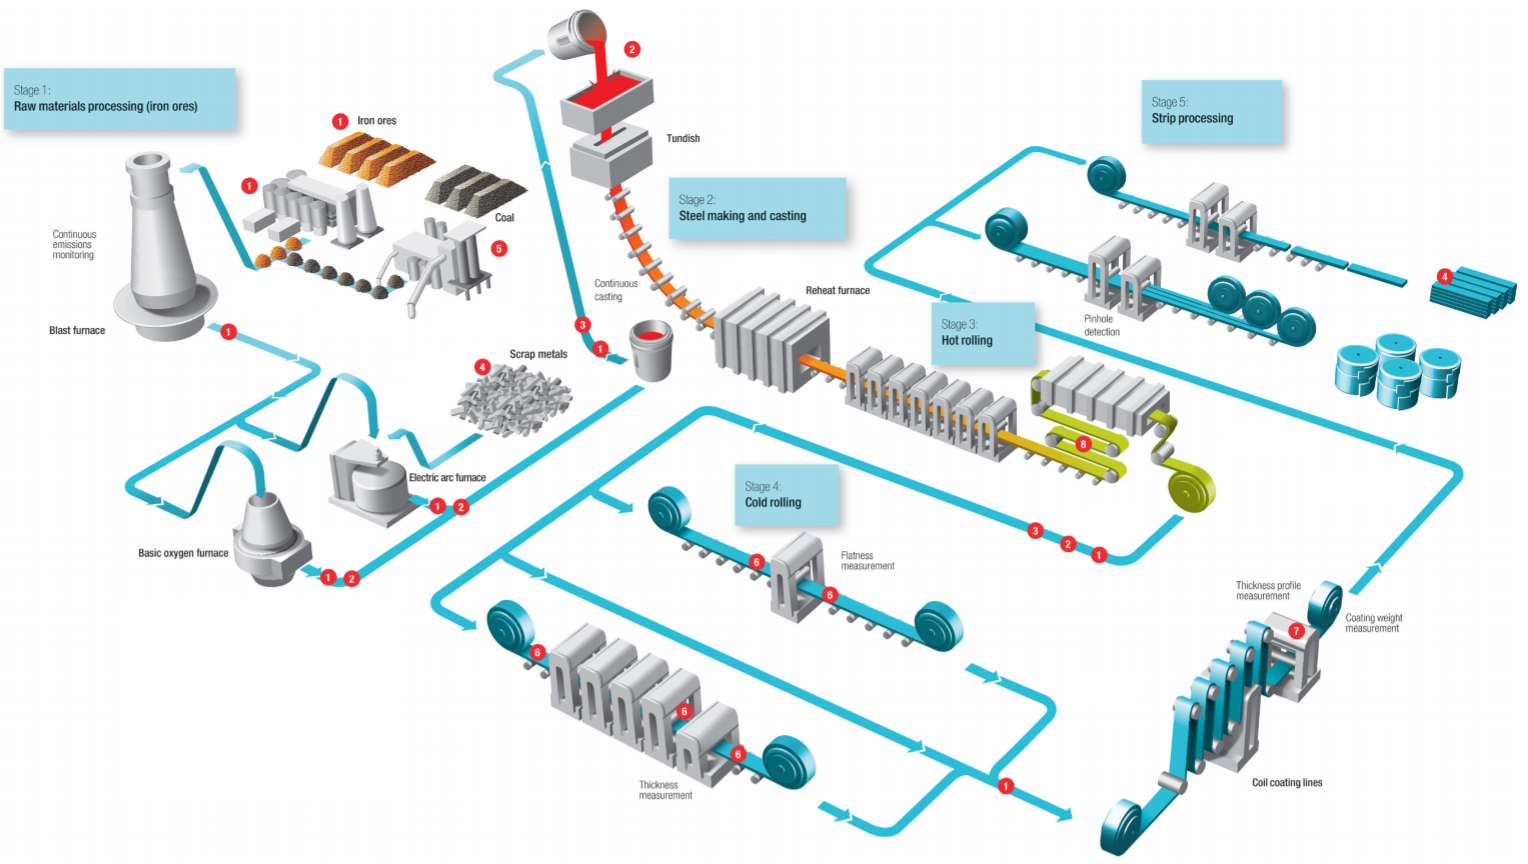
\includegraphics[width=1.0\linewidth]{../images/steel-production-steps.png}}
		\caption{Steel Manufacturing Steps~\cite{sinha-spinks_2015}.}
		\label{figure-steel-production-steps}
	\end{center}
\end{figure}
	
	A steel manufacture facility's production lines might be structured with different combinations of those steps based on the diversity of the demanded output product or the manufacture facility capacities. 'Production Constraints' which is a critical subject to optimization researches arise from those technology-driven production types related to facility capabilities~\cite{cowling2001design}. Raw materials like coal, iron ores, and scrap metals are melted in blast/electric arc/basic oxygen furnaces to obtain liquid iron as primary product. Accordingly, liquid steel alloy is sent to a continuous casting line, and poured into a large customized volume trapezoid prism called tundish. The steel alloy comes off the mold close to the bottom outlet of the tundish and gets into an entry nozzle until it reaches the rollers. The shaped material is treated between rollers with a water cooling system, and converted into semi-finished casting products such as slabs, blooms, or billets. For the purpose of gaining the desired mechanical properties, uniform thickness of the material, and controlling width dimension, outputs are sent to the rolling process which is a pressing application on slabs by using rolls. The rolling process can be performed in two different modes: hot rolling and cold rolling. Hot rolling can be performed if the material temperature is above its re-crystallization temperature. Otherwise, reheat furnaces are used to obtain the proper temperature of the metal which is known as deformation temperature prior to the hot rolling process. Metals with a material temperature below re-crystallization temperature are treated in a cold rolling process. Surface finish and flatness can be improved and modification of material work hardening can be achieved with the cold rolling process. With the coiling step in the rolling process, slabs might be converted into compact coils featuring high lengths unless they will not be sent to further steps on the continuous production line. The following steps can be given as pickling process and hot-dip galvanizing process. As an effective coil coating technique, galvanizing is an application of protective zinc coating on the steel surface to improve corrosion resistance. If this method is applied by submerging the steel parts into a molten zinc bath, it is called hot-dip galvanizing process. Considering the roughly explained production steps above, each process has its own technical or physical constraints. Optimizing individual sequences in each process is a necessity for a successful local process. Local constraints on different processes are integral parts of a global optimization problem that is tackled by human expert planners for a solution. The sequences produced in production lines are available as data output, so-called 'imprints' of what has been on sequence designers' mind. Therefore, looking at the historical production data, and an investigation on the properties of those order sequences that have already been produced give indirect access to the patterns which are related to human experts' knowledge system. The technical and physical constraints mentioned in the introduction section are obviously unique to those specific production lines and they vary under differently customized production lines. Produced order properties such as thickness, width, temperature, and chemical composition are the characteristic features of order products that are possibly shaped under the effect of those constraints. An investigation on the features of orders in the same production sequences and comparison between them might give interesting clues about related constraints and correspondingly provide patterns about human experts' decision strategies.
		
	I should discuss and refer to different constraints from the literature introduced for the manufacturing life cycle.
	
	As a motivation, I need to introduce different categories of constraints as technical constraints, performance-indicator based constraints to be quantified in the context of the FBA in the further steps of this work.
	
	Are logistic constraints, physical and chemical constraints coupled to topological features of the association network?
}

\section{Research Objective}

{\color{red} 
	Our hypothesis: different types of constraints create non-random features in the association networks for different binning schemes. Networks derived from various types of binning. Do they show non-random features when I have performance constraints or other types of constraints?
	
	Explanation of my hypothesis is a theoretical/conceptual framework as a starting point for the investigation. It is a well-defined valid object and based on facts. Moreover, it is structured to discriminate the two types of constraints in the statistical properties of the production data.
	
	The initial step of this master thesis work was to quantify the characteristics of two hypothetical types of constraints in industrial production: technology-driven constraints and load-driven constraints. 
}

\section{Research Plan and Thesis Organization}

{\color{red} 
	Methods are introduced here as indicative of two fundamentally different constraints acting on the manufacturing process: technological constraints on the one hand and constraints related to material flow and production capacity on the other.
	
	I plan to quantify the characteristics of two hypothetical types of constraints with an Operations Research Model consisting of two steps. First, analyzing the statistical properties of association networks over Time in an extensive data set from steel manufacturing; second, developing an abstract theoretical framework to understand better the connection between each type of constraint and the statistical patterns created by them. 
	
	Formulate the binning methods here because this will describe the hypothesis underlining my thesis.
	
	My Operations Research Model (OR model) combines Steel Manufacturing Events Analysis and Flux Balance Analysis. The art form of this model is to structure a standard data format and a shared analysis logic that allows comparing the results from manufacturing data and simulation data.
}